\documentclass[12pt,a4paper]{article}
\usepackage{graphicx}
\begin{document}
	\begin{titlepage}
		\centering
		\vspace*{\fill}
		
		\vspace*{0.5cm}
		
		\huge\bfseries
		\rule{\textwidth}{1.6pt}\\[\baselineskip]
		Thutong Site Learning Center User Manual
		
		\vspace*{0.5cm}
		
		\large Edited by: \\[\baselineskip]
		
			{Fiwa lekhulani\\Daniel Rocha\\lebogang Ntatleng\\Lesego Mabe\\Tlou Lebelo\\Oluwatosin Botti}
		
		\rule{\textwidth}{1.6pt}\\[\baselineskip]
		
		
		\vspace*{\fill}
	\end{titlepage}

	\section{Product Overview}
		The Thutong Site Learning Center is an online system intended for high school students. It is aimed at providing students with online material to catch up on any content that they might have missed in class or did not comprehend during class. it is also aimed at providing teachers a way of uploading course content to the system for students to go through, and provide quizzes for the students to test their knowledge after the completion of a topic. 
	
	\section{System Configuration}
		The Thutong Site Learning Center system need not be installed on any any digital device, it is available online. The system can be accessed through desktop computers and mobile devices and users will need a network connection in order to have access to it. The image below is a graphical depiction of the communication between users and the system, including the protocols used between the two entities.
		
		%NOTE:please load an image here!!!
		
	\section{Installation}
		The system does not need to be installed as mentioned above, the user need only have a digital device with an internet connection and a web browser.
		
	\section{Getting Started}
		The Thutong system is aimed at improving South Africa's Science ratings, this means that it is intended to be used by every student in South Africa, thus it is free and no license is needed to use it.\\
		There are 4 types of users in the Thutong system, these are:
		\begin{itemize}
			\item Students
			\item Expert Consultants(Teachers)
			\item Marketing Consultants
			\item Administrator
		\end{itemize} 
		  
		\subsection{The student}
		 The first user of the system is the student. This user needs to login with either their google, facebook or email account in order to access any content from the system. The student also needs to be able to search for a specific subject and be able to view content within that subject. Only one of the login options is shown above, which is registration before login\\
		 
		 %imagee to be loaded here(screenshot)
		 
		 \begin{figure}
		 	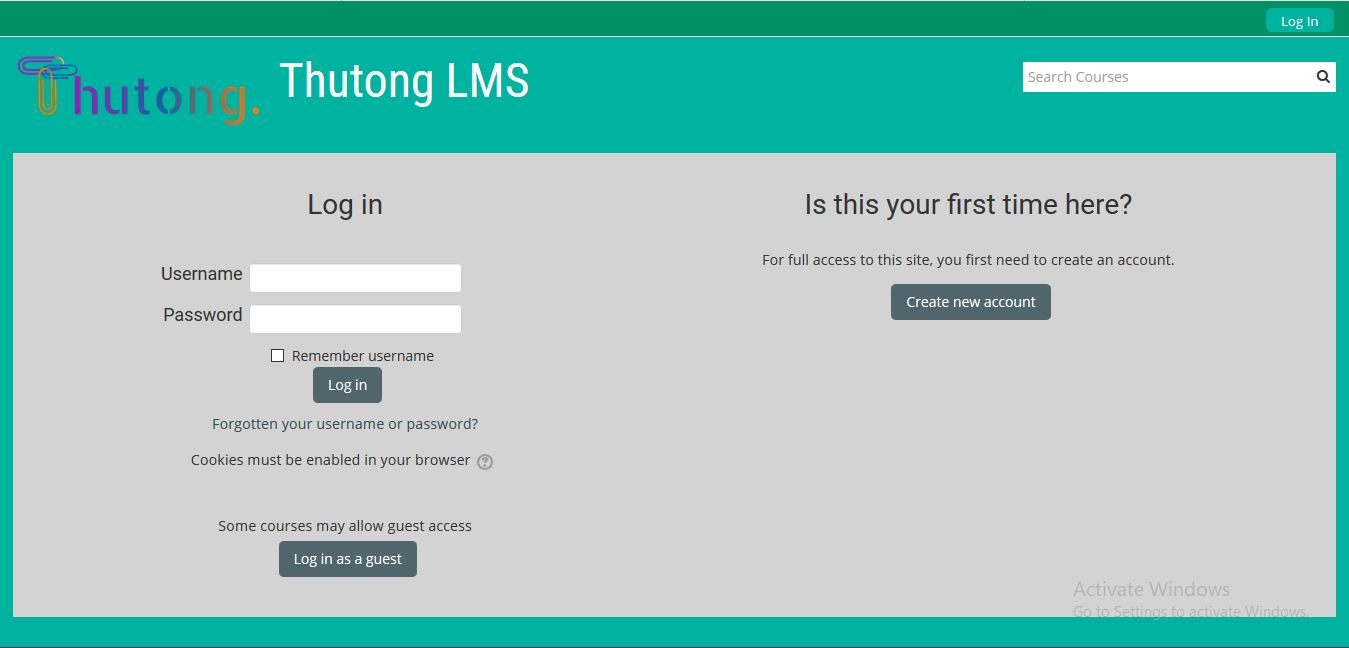
\includegraphics[width=\linewidth]{login.jpg}
		 	\caption{User Registration and Login.}
		 	\label{fig:user login}
		 \end{figure}
		 
		 \subsection{The Expert Consultant}
		 The Expert consultant needs to be able to, besides logging in, add course content intended for students on the system. They should also be able to create quizzes for students and be able to remove all of the above-mentioned entities. Figure 1 also shows on the right pane, the expert consultants registration, which will need to be validated by the administrator.
		
		\subsection{The Marketing Consultant}
		 This user needs to be able to add, remove and update marketing content on the system like vacancies, advertisements and donation request. A depiction of their interaction with the system is shown below.
		 
		 
		 \subsection{The Administrator}
		 Also known as the superuser, this user will have all the powers of all the users, and will also be responsible for the addition, validation and removal of Expert and Marketing consultant accounts since these two users may be outsourced throughout the lifetime of the system. An example of the Admin interacting with the system is shown below.
		 
	\section{Using the System}
	 This section discusses the use cases of the system in detail, please refer to the subsections below for each use case by the various users of the system.
	 	\subsection{Login}
	 	 From figure (d) below, the user is welcomed by the home oage and then enters their details to login.
	 	 
	 	 \subsection{Searching for a course or subject}
	 	 To search for a specific course or subject, the user enters text in the textbox on the left and then clicks search, they will then be taken to Figure 3 where they enter whatever topic they which to search for, and the result will be displayed in Figure 4 below.
	 	 
	 	 
	 	 
	 	 \subsection{Adding a course or subject}
		 As seen on Figure 5 below, adding a course or subject requires the subject name, description and which grade it is intended for. 
		 
		 
		 
		 
		 
		 
		 
		 
		 \begin{figure}
		 	\includegraphics[width=\linewidth]{Home.jpg}
		 	\caption{home page}
		 	\label{fig:home page}
		 \end{figure}
		 
		 \begin{figure}
		 	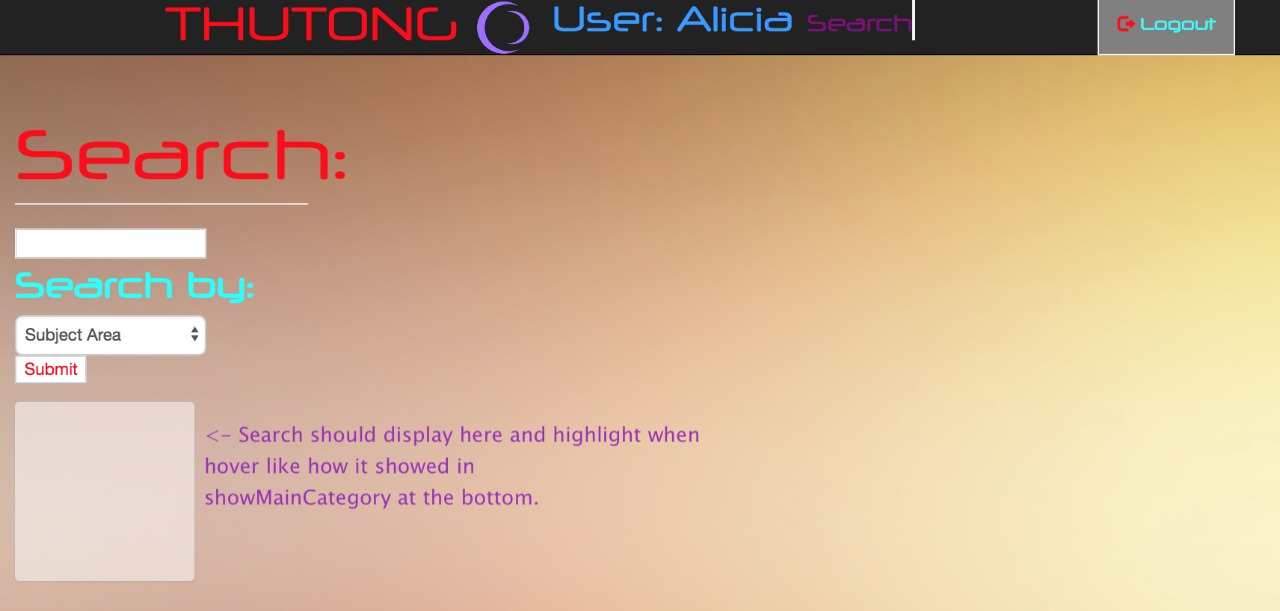
\includegraphics[width=\linewidth]{Search.jpg}
		 	\caption{Search}
		 	\label{fig:Searching for subject}
		 \end{figure}
	 
	 	\begin{figure}
	 		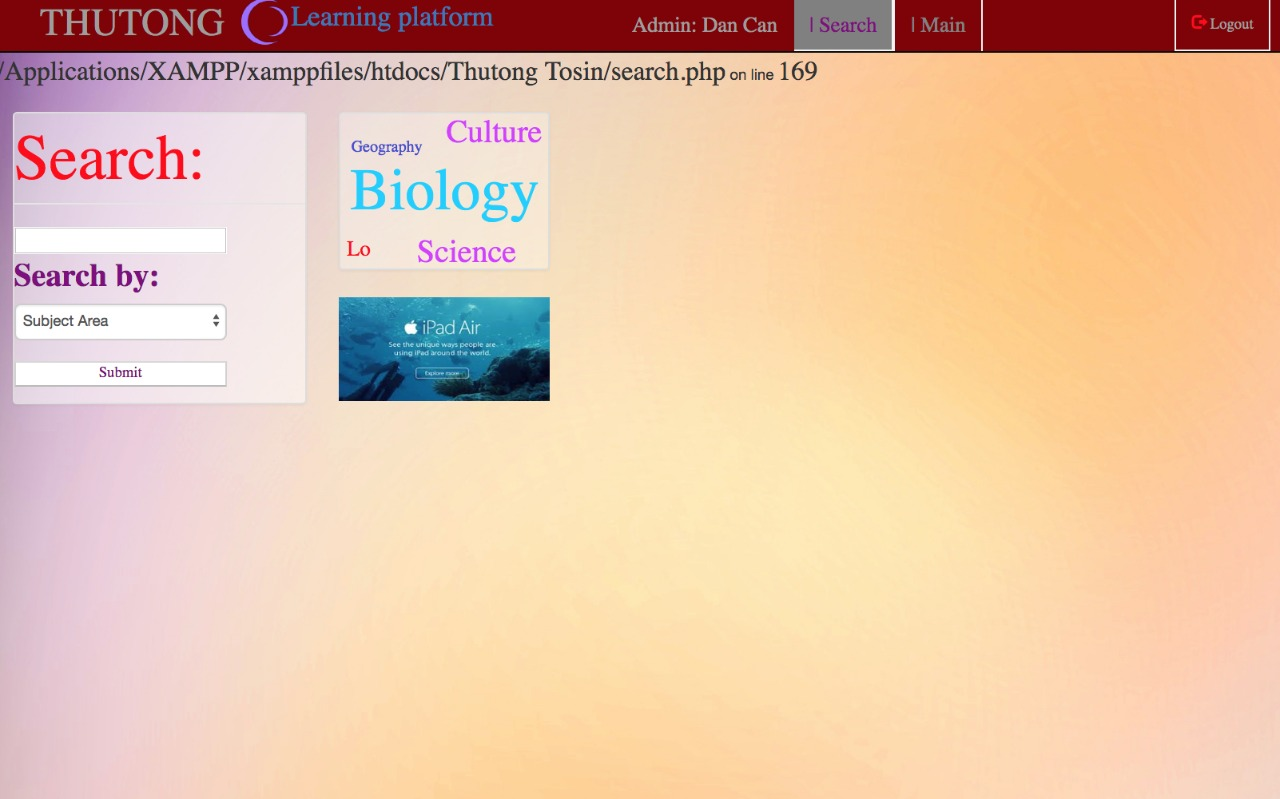
\includegraphics[width=\linewidth]{Search2.jpg}
	 		\caption{Search}
	 		\label{fig:Searching for subject continued..}
	 	\end{figure}
 	
 		 \begin{figure}
 			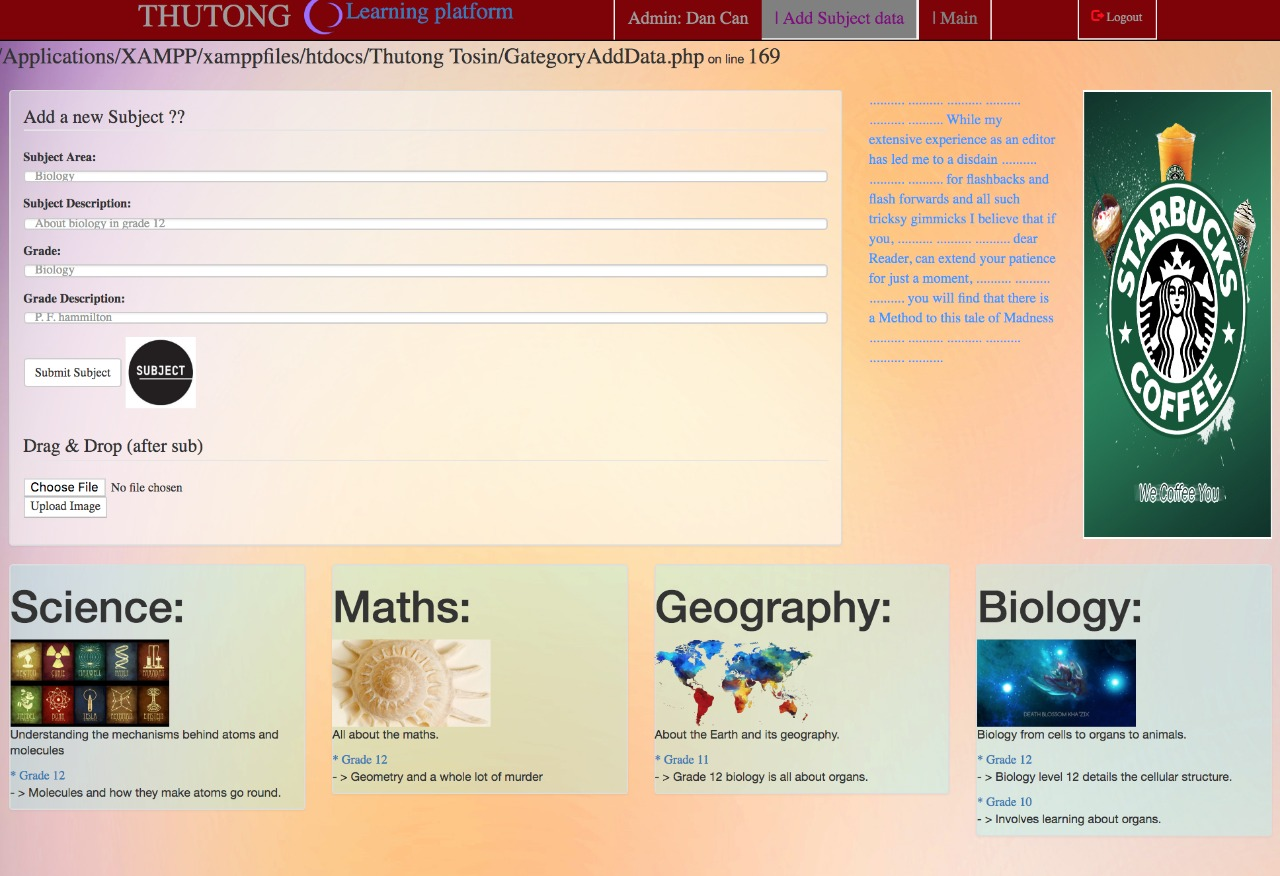
\includegraphics[width=\linewidth]{AddSubject.jpg}
 			\caption{adding a subject}
 			\label{fig:Adding a subject or course}
 		\end{figure}
	
\end{document}
